\documentclass[a4paper,10pt]{article}
\usepackage{linuxtag,graphicx,times}
\usepackage[english]{babel} % or german/ngerman
\usepackage{isolatin1}      % isolatin input encoding for convenience
\usepackage{epsfig}         % this is how we're doing pictures
\selectlanguage{english}    % or ngerman for german language
\pagestyle{empty}% Requirement: No page numbers

\title{\Large\textbf{%
The FlightGear Flight Simulator\\
History, status and future
}}

\author{A.R. Perry \textsl{$<$alex.perry@ieee.org$>$}\\
        C. Olson \textsl{$<$curt@flightgear.org$>$}\\
        \textsl{http://www.flightgear.org/}}
\par\date{}\par
\begin{document}
\renewcommand{\thepage}{}
\twocolumn[%
\pagestyle{empty}
\maketitle
\pagestyle{empty}

\begin{center}
\begin{abstract}
\vspace*{.5\baselineskip}
\parbox{0.66\textwidth}{%
%
\hyphenpenalty1000000 
The open source flight simulator \textsl{FlightGear}
is being developed through gracious
contributions of source code
and time by many talented people from around the globe.
%
The main focus of this project is a desire to `do things right',
to minimize short cuts, to learn and advance knowledge
and to have better toys to play with on ordinary computers.
%
}
\end{abstract}
\end{center}

] % end of single column part in twocolumn document

\sloppy\hbadness 9999
\hyphenpenalty2000
%
%%%%%%%%%%%%%%%%%%%%%%%%%%%%%%%%%%%%%%%%%%%%%%%%%%%%%%%%%%%%%%%%%%
%
% * Introductory History
%
In April 1996, David Murr, drawing on ideas
brought forth by others, proposed a new flight simulator developed by
volunteers over the Internet. This flight simulator was to be
distributed free of charge via the Internet and similar networks.

Curt Olson made a multiplatform release of FlightGear\cite{fgfs} in July 1997.
Since then, it has expanded beyond flight aerodynamics by improving graphics,
adding a shaded sky with
sun, moon and stars correctly drawn, automatically generated worldwide
scenery, clouds and fog, head up display and instrument panel,
electronic navigation systems, airports and runways, network play,
and much more (as shown in figure \ref{fig:c172}).

How does it all work ?
%
%%%%%%%%%%%%%%%%%%%%%%%%%%%%%%%%%%%%%%%%%%%%%%%%%%%%%%%%%%%%%%%%%%
%
% At the beginning, a pretty yet pointless screenshot
%
\begin{figure}
\begin{center}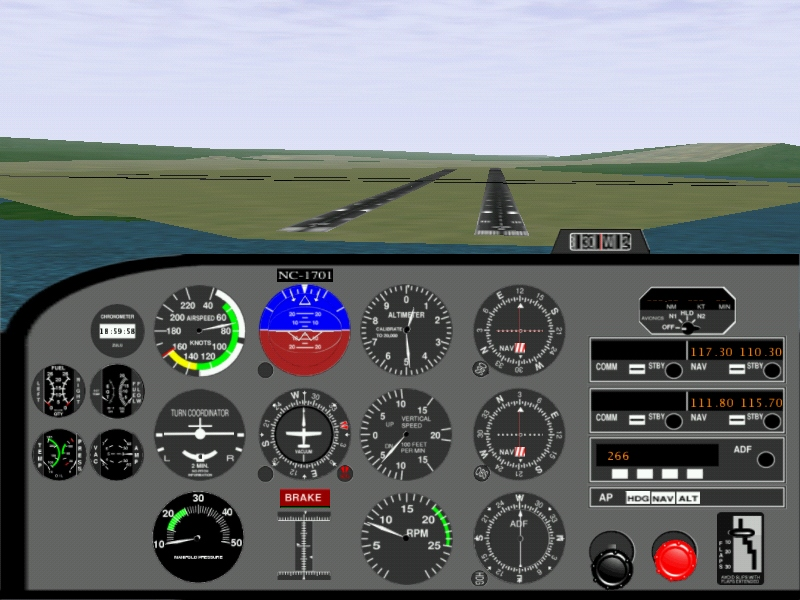
\epsfig{file=c172.eps,width=8cm}\end{center}
\caption{Cessna 172 on landing approach}
\label{fig:c172}
\end{figure}
%
%%%%%%%%%%%%%%%%%%%%%%%%%%%%%%%%%%%%%%%%%%%%%%%%%%%%%%%%%%%%%%%%%%
%
\section*{Simulator Portability}

FlightGear aims to be portable across many different processors and
operating systems, as well as scale upwards from commodity computers.
In addition to endianness, which inconveniences most open source projects,
we must also use services (such as sound) whose implementation may be
equivalent, yet very different, under the various operating systems.
For those services which are common across most video games, the
\textsl{PLIB} project offers a simple API that acts as a
\textbf{P}ortable \textbf{Lib}rary\cite{plib}.
Some aspects, such as sound support, generate libraries that implement
the functionality.  Other aspects, such as joystick support, are able
to declare an object in a single header file and thereby avoid the library.

Compared to Windows, MacOS and Irix, the various distributions and releases
of Linux-based operating systems are very similar.  There are important
differences, most of which cause problems when trying to build and test
\textsl{PLIB}, so these rarely impact FlightGear directly.
With joysticks, for
example:
\begin{enumerate}
\item The kernel provides two methods for retrieving input data,
the newer one permits more axes and buttons
\item Distributions disagree on whether the {\tt js*} files
should reside in a subdirectory under {\tt /dev}
\item Autodetection of serial and gameport devices often occurs at boot,
earlier than users expect
\item Hot-swap support for USB does not assign predictable devices,
so the yoke and rudder pedals are sometimes exchanged
\end{enumerate}

% * Compatibility issues with distributing linux binaries
%
Once the facilities required by video games are available through
the Portable Library, the remainder of the code acts as a conventional
application.  Compile-time incompatibilities are primarily due to
{\tt gcc} versioning and installing libraries without their header files.
Run-time problems are rare,
if \textsl{PLIB}'s example code was used as test cases.

Any linux user can download the source, compile it and
safely expect it to run.
Unfortunately, you generally cannot short-cut
this process by copying someone else's binary.
This is a generic problem, encountered by many applications,
and led to the \textsl{Linux Standards Base} project\cite{lsb}.

It is made many times worse for FlightGear because
hardware differences force library selections
to be modified so that a given binary may not even be usable on
another machine with the same Linux distribution and release
if it has a different graphics card (for example).
This is especially true with GL support, the extensions, and the
level of GLX implementation available.  This is being addressed
by the \textsl{Linux OpenGL Application Binary Interface}
(ABI)\cite{abi}.
%
%%%%%%%%%%%%%%%%%%%%%%%%%%%%%%%%%%%%%%%%%%%%%%%%%%%%%%%%%%%%%%%%%%
%
\section*{Simulator Structure}
%
Current commercial PC flight simulators are proprietary,
lack extensibility and thus are resistant to
modification and enhancement.  If the FlightGear project
wishes to fill the gap, it must provide a flexible framework.

% * Modules and object oriented structure of source code

The FlightGear source tree is only one level
deep, except that all the flight data models are each in
their own subdirectory located under the
FDM directory.
Each directory contains a few header files that expose its object
definitions.  Other source files refer to the headers directly,
without path globbing or multiple include paths for the compiler.
The directory names are mostly pretty self-explanatory:

Aircraft,
Airports,
Autopilot,
Time (in the simulated world),
Cockpit,
Controls (in the aircraft cockpit),
FDM (only one constituent in use),
GUI (menus and the like),
Include (for compiler configuration),
Joystick,
Main (initialization and command line parsing),
Network (data sharing),
NetworkOLK (network play),
Objects (dynamically loaded and changing scenery),
Scenery (static),
Weather (world wide basic factors),
WeatherCM (four dimensional world database),
Navaids,
Ephemeris (of celestial bodies) and
Sound.

In addition to the collection of interacting objects, FlightGear
also exposes the high level state of the simulation in two ways.
First, a meta-object \textsl{BFI} provides a long list of
methods to retrieve (and, in some cases, modify) popular information that
is distributed around the many different types of objects.
This avoids making each source file dependent on the declarations
of almost every object type and header file.  These references
and interactions can only really be modified at compile time.

The second exposure of the simulator state occurs through the
property database, which dynamically maps a name (such as 
\texttt{/position/latitude}) into an object with getter
and setter methods.  Although slower, the dynamic access is
especially appropriate for the user interface, parametric graphics
elements and configuration files.

The property database is also exposed
to other applications by the network interface.
The command line option \\
\texttt{--props=socket,bi,20,,5555,tcp},
for example, allows someone else (such as the flight instructor)
to run \texttt{telnet localhost 5555}.  This allows
arbitrary properties to be viewed and modified while
the simulation is running.  

Many tasks within the simulator need to only run periodically. These
are typically tasks that calculate values that don't change
significantly in 1/60th of a second, but instead change noticeably on
the order of seconds, minutes, or hours.
Running these tasks every iteration would needless degrade
performance. Instead, we would like to spread these out over time to
minimize the impact they might have on frame rates, and minimize the
chance of pauses and hesitations.

We do this using the \textsl{Periodic Event Manager and Scheduler},
which consists of two parts. The first part is simply a list
of registered events along with any management information associated
with that event. The second part is a run queue. When events are
triggered, they are placed in the run queue. The system executes only
one pending event per iteration in order to balance the load.
The manager also acquires statistics about event execution
such as the total time spent running this event, the quickest run, the
slowest run, and the total number of times run. We can output the list
of events along with these statistics in order to determine if any of
them are consuming an excessive amount of time, or if there is any
chance that a particular event could run slow enough to be responsible
for a perceived hesitation or pause in the flow of the simulation.
%
%%%%%%%%%%%%%%%%%%%%%%%%%%%%%%%%%%%%%%%%%%%%%%%%%%%%%%%%%%%%%%%%%%
%
\section*{Simulator Execution}
%
% * Procedure for building and installing from source
%
Installing and running FlightGear is relatively easy under Linux,
especially compared to other operating systems with weak tool automation.
\begin{enumerate}
\item Install Linux normally and test internet access.
\item Add video card support, using a maximum of 25\% of memory for 2D display.
\item Enable hardware accelerated OpenGL support and test for speed,
using \textsl{glTron}\cite{gltron} for example.
\item Install \textsl{PLIB} 1.2 or above,
which is already in many distributions,
and test with all the supplied examples to ensure the API is working.
\item Download, compile and install \textsl{SimGear}.
If your distribution already 
includes some components, such as
\textsl{zlib}, verify that headers are present.
\item While that compiles, download the FlightGear source.
Once \textsl{SimGear} is installed, start the compile and then install it
\item While the simulator is compiling, download FlightGear's base package.
This contains data files that are required to execute the binary application.
\item Type {\tt runfgfs} and enjoy.
\end{enumerate}

For a computer system which is directly supported by your chosen distribution,
the first five steps are often trivialized into telling the installer to 
ensure `plib-dev' is present.
Starting from a blank hard drive,
FlightGear can be running in less than an hour.
%
%%%%%%%%%%%%%%%%%%%%%%%%%%%%%%%%%%%%%%%%%%%%%%%%%%%%%%%%%%%%%%%%%%
%
\section*{Simulating the Pilot}
%
The new FlightGear pilot will probably not want to remain within the San
Francisco bay area, which is the small scenery patch included in the 
Base package.
The scenery server allows the selection and retrieval of any region of the
world.  Joining other users in the sky is another possibility.

% * multiple user capabilities
%
In a large group of users, coordinating the position and activities of
all the players requires considerable network traffic, which can degrade
the apparent performance.
The FlightGear Deamon, \texttt{fgd}, is a standalone program which can
run on a separate computer that is independent of any FlightGear session.
It registers FGFS players
willing to take part in a multiplayer FGFS environment via TCP/IP.
Information like the player's IP/lon/lat/alt and inter-player
messages can be sent to \texttt{fgd}, 
which in turn sends back the gathered information upon request.
In this way, the simulated aircraft all become visible to each other.

Due to limited monitor size, the view that is available on a normal
computer is more like the little passenger portholes on airlines
and a poor substitute for the wraparound windows of general aviation
aircraft.  This is especially true when the simulated aircraft has
an open cockpit and an unrestricted view in almost all directions.
%
\begin{figure}
\begin{center}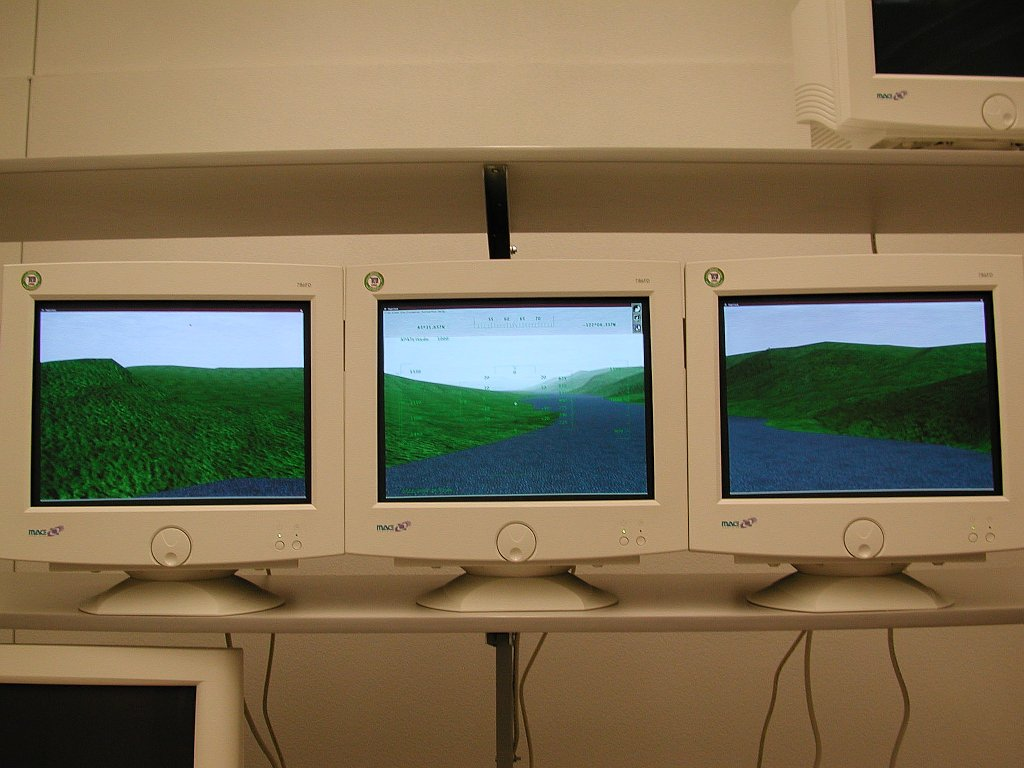
\epsfig{file=threevid.eps,width=8cm}\end{center}
\caption{Panoramic scenery}
\label{fig:threevid}
\end{figure}

% * multiple display capabilities
%
To alleviate the problem with lack of external view, FlightGear
supports synchronizing several displays together to form a panoramic
or wrap around view.

FlightGear has built in support for network socket communication and
the display synchronzing is built on top of this support.  FlightGear
also supports a null or do-nothing flight model which expects the
flight model parameters to be updated somewhere else in the code.
Combining these two features allows you to synchronize displays.

For example, let's assume we want to setup the example shown in figure
\ref{fig:threevid}.

\begin{enumerate}
%
\item Ideally, configure three identical computers and monitors.
%
\item Pick one of the computers (i.e. the center channel) to be the
master.  The left and right will be slaves \textsl{s1} and \textsl{s2}.
%
\item When you start \texttt{runfgfs} on the master,
use the command line options \\
\texttt{--native=socket,out,60,s1,5500,udp} \\
\texttt{--native=socket,out,60,s2,5500,udp}
respectively to specify
that we are sending the ``native'' protocol out of a udp socket channel
at 60~Hz, to a slave machine on port 5500.
%
\item When you start \texttt{runfgfs} on each of the slave computers, 
use the command line
option \texttt{--native=socket,in,60,,5500,udp} to
specify that we expect to receive the native protocol via a udp
socket on port 5500.  The second option
\texttt{--fdm=external} tells the slave not to run
it's own flight model math, but instead receive the values from an
``external'' source.
%
\item You need to ensure that the field of view on the scenery
matches the apparent size of the monitor to the pilot.
\texttt{--fov=xx.x} allows you to specify the field of view in degrees
on each computer display individually.
%
\item \texttt{--view-offset=xx.x} allows you to specify the view offset
direction in degrees.  For instance,\\
\texttt{--view-offset=0} for the center channel,\\
\texttt{--view-offset=-50} for slave 1, and\\
\texttt{--view-offset=50} for slave 2.
%
\end{enumerate}

There is no built in limit to the number of slaves you may have.  It
wouldn't be too hard to implement a full 360 degree wrap around
display using 6 computers and 6 projectors, each covering 60 degree
field of view on a cylindrical projection screen.

%%%%%%%%%%%%%%%%%%%%%%%%%%%%%%%%%%%%%%%%%%%%%%%%%%%%%%%%%%%%%%%%%%
%
\section*{Simulating the Aircraft}
%
% * Generic flight data model - JSBsim
%
The aerodynamic simulation may be only one constituent of the whole
environment being simulated for the user, but its performance is
critical to the quality of the user's simulation experience.
Errors in this \textsl{Flight Dynamics Model} (FDM) are distracting
to the pilot.
Other simulator components, such as the autopilot,
are designed to expect a realistic
aircraft, may respond incorrectly as a result of FDM errors
and provide additional pilot distractions. These factors
can ruin the immersive experience that the user is seeking.

As a result of this concern, FlightGear abstracts all of the
code that implements an FDM behind an object oriented interface.
As future applications find that existing FDM choices do not meet
their requirements, additional FDM code can be added to the project
without impacting the consistent performance of existing applications.

The original FDM was LaRCsim, which models a Cessna 172 using
dedicated C source that has the necessary coefficients hard coded.
It is sufficient for most flight situations that a passenger would choose
to experience in a real aircraft.  Unusual maneuvers that are often
intentionally performed for training purposes are poorly modelled,
including deep stalls, incipient and developed spins and steep turns.
The code also supports a Navion and a Cherokee, to a similar quality.

A research group at the University of Illinois created a derivative
of LaRCsim, with simplified the models such that they are only
really useful for cruise flight regimes.  They enhanced the code with
a parametric capability, such that a configuration file could be
selected at simulation start to determine how the aircraft will fly.
Their use for this modification was to investigate the effect on
aircraft handling of progressive accumulations of ice.
%
\begin{figure}
\begin{center}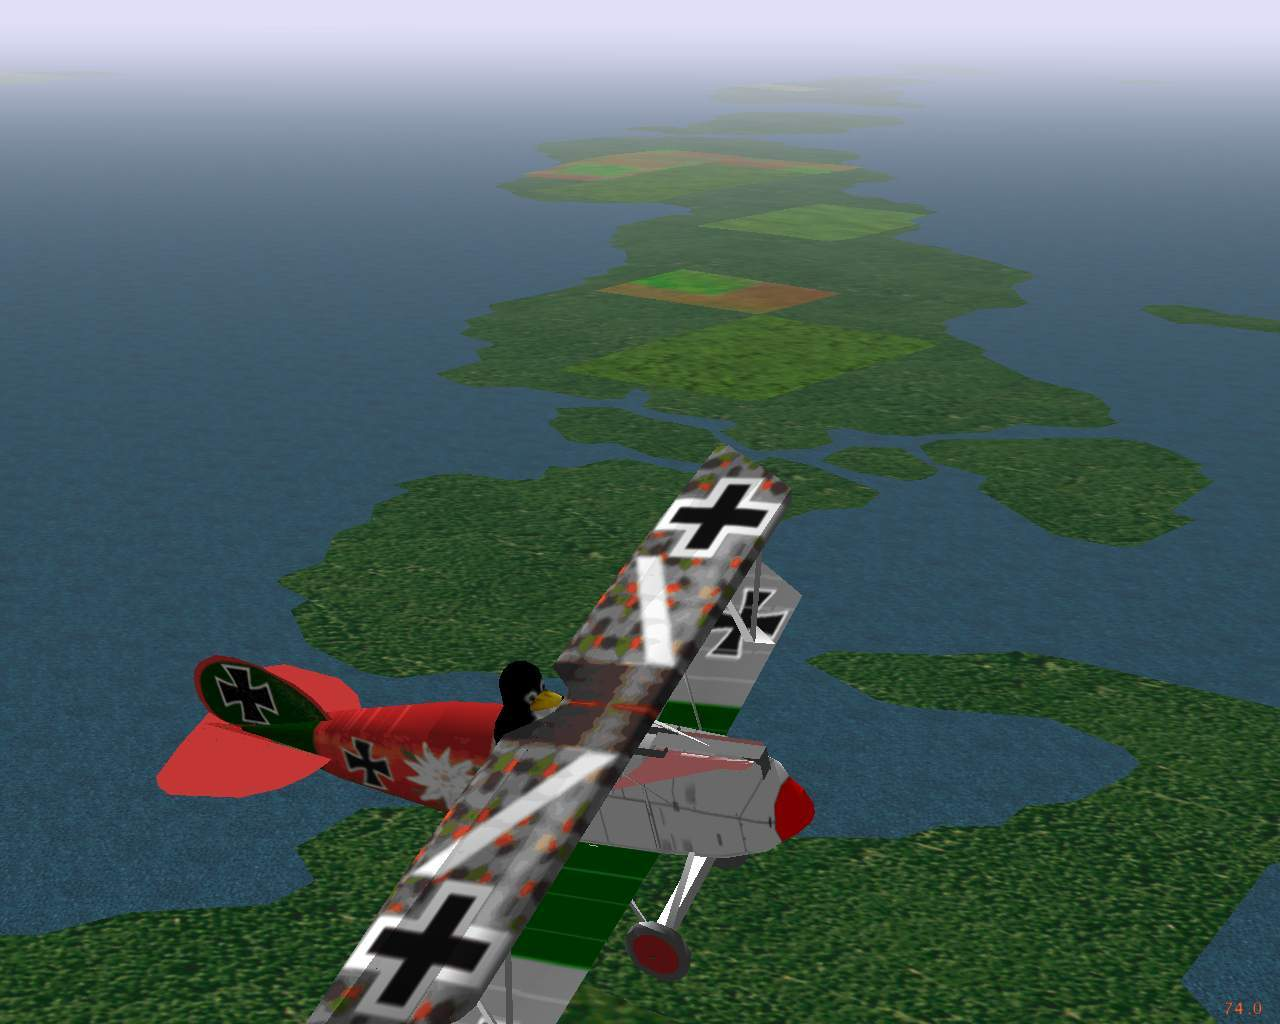
\epsfig{file=wh-tux.eps,width=8cm}\end{center}
\caption{Tux flying over Woods Hole}
\label{fig:wh-tux}
\end{figure}

Another group is developing a completely parametric FDM code base,
where all the information is retrieved from XML format files.
Their JSBSim project\cite{jsbsim}
can run independently of a full environmental
simulation, to examine aerodynamic handling and other behavior.
An abstraction layer links the object environment of FlightGear
to the object collection of JSBSim to provide an integrated system.
Currently, this FDM supports the Cessna 172 and the X-15 (a hypersonic
rocket propelled research vehicle), providing the contrast between an
aircraft used for teaching new student pilots and an aircraft that
could only be flown by highly trained test pilots.

% * User modifiable XML configuration support

The rest of FlightGear's configuration files are also moving towards
XML, such as the engine models,
the instrument panel layouts and instrument design, the HUD layout,
the user preferences and saved state.
The real benefit of using XML here is that people with no software
development experience can easily and effectively contribute.
Pilots, instructors, maintenance technicians and researchers all have
in-depth technical knowledge of how 
an aircraft and hence the simulator should behave,
so it is critical that we allow them direct access to the internals.

Both the head up display (HUD) and the instrument panel allow
the user to specify an XML file describing which instruments
are to be displayed and where they should be located on-screen.
Individual instruments are defined in independent XML files,
selecting graphic elements, texture bitmaps and transforms that modify
these to build the desired effect.  Some of the transforms are fixed
and others are parametric on simulator data, so that the rotation 
angle of a needle bitmap on the airspeed instrument is determined
by the computed airspeed value inside the FDM section of the simulator.

% * Instrument panel and HUD
%
The head up display of a real aircraft uses computer generated
graphics, so the software can generally detect, and correct for,
the flaws and inaccuracies in the sensors that are feeding it data.
As a result, the information presented to the pilot is generally
accurate.  Simulating that is relatively easy, since the actual
state of the aircraft can be retrieved and directly displayed.

An important aspect of learning
to fly an aircraft (without computer assistance) is understanding
what the limitations and errors of the various instruments are,
and when their indications can be trusted as useful flight data.
Unfortunately, the information from panel instruments has errors,
which in general only read a single sensor value
with negligible correction for the
limitations of the sensors being used.  
When the FlightGear panel advanced from no errors to having only
two of the limitations implemented, the non-pilot developers went
from trivially flying instrument approaches to frequent ground impacts.

Considerable effort is needed to write this code.  Gyroscopes can
slow down and wobble, their rotation axis can drift, they can hit
gimbal stops and tumble and their power source can be weak or fail.
Air-based instruments are wrong in certain weather conditions,
tend not to respond immediately, can be blocked by rainwater in the
lines, or become unusable when iced over.  Radio navigation is
subject to line-of-sight, signals bounce off hills and bend near
lake shores or where another aircraft is in the way and
distant stations can interfere.  Still more errors are associated
with the magnetic compass, and other instruments that seem 'trivial'.

Currently, the communication radios are not implemented, so that pilots
cannot use their microphone inputs to interact.  Radio usage is a large
part of the complexity in operating at large and busy airports.
Unfortunately, this often
encourages pilots to fly the microphone and forget about the airplane,
occasionally with disastrous results.  We hope to implement this feature
soon, to provide another source of challenging distractions to the pilot.
%
%%%%%%%%%%%%%%%%%%%%%%%%%%%%%%%%%%%%%%%%%%%%%%%%%%%%%%%%%%%%%%%%%%
%
\section*{Simulating the World}
%
The purpose of the TerraGear project\cite{terragear}
is to develop open-source tools and
rendering libraries and collect free data for building 3D
representations (or maps) of the earth for use in real time rendering
projects.
There is much freely available 
\textsl{Geographic Information System} (GIS) data on the
internet.  Because the core
data for FlightGear has to be unrestricted,
the default use of the project only uses source data that doesn't
impose restrictions on derivative
works.  Three categories of data are used.

Digital Elevation Model (DEM) data 
is typically a set of elevation points on a regular grid.  Currently,
30 arcsecond (about $1\,km=0.6\,mi$) data for the whole world,
and 3 arcsecond (about $100\,m=300\,ft$) data for the United States,
is available from the USGS, but better data sources are hoped for.
An optimizing algorithm seeks to find the smallest number of flat
triangles that provide a fairly smooth and realistic terrain contour.
This algorithm reduces the number of triangles need to render an area
while preserving all the detail within some specified error tolerance.

Other more specialized data such as airport beacon,
lighthouse locations, radio transmission towers
and the like are available
in listings from various government agencies.  These generally provide
a short text description of the item and its geographic coordinates.
The challenge is to convert each entry into a realistic visual object
which can be inserted into the scenery database.

Polygonal data such as landmass outlines, lakes, islands, ponds, urban
areas, glaciers, land use and vegetation are available from the USGS
and other sources.  The GSHHS database provides a highly detailed and
accurate global land mass data so we can model precise coast lines for
the entire world.  Based on the source of the data and factoring in
the land use data, we can select an appropriate texture which will be
painted onto the individual triangles.  Where necessary, triangles are
subdivided to get the effect correct.  Runways and taxiways are
generated by converting the list of runway segments into polygons,
painted with appropriate surface texture and markings, and then
integrated into the scenery in the same way.

Clearly, someone can gain access to data sources that are under
more restrictive licenses, use the TerraGear project tools to generate
enhanced scenery and then distribute those files as they choose.
Both the FlightGear and TerraGear projects encourage this kind
of enhancement, because the basic open source packages cannot do this.

% * Trade-offs for world wide visual scenery  - TerraGear
%
There is a trade-off between the quality of the scenery and the speed
at which it can be rendered by the graphics card.  As cards get faster,
it becomes feasible to place more detail into the scenery while maintaining
a useful and smooth visual effect.
There are many techniques for adjusting the level of detail according to
the altitude and attitude of the aircraft, to optimize the visual quality,
but none of them are currently implemented as they cause visual artifacts.

Currently, the visual effect is clearly
synthetic, as can be seen in figure \ref{fig:wh-tux}, 
but it has sufficient information to readily permit navigation by
pilotage (i.e. comparing the view out of the window to a chart).
The compressed data requires about one kilobyte per square kilometer.
All the information inside the scenery database is arranged in a
four-level hierarchy,
where each level changes scale by a factor between 10 and 100:

\begin{figure}
\begin{center}\epsfig{file=theworld.eps,width=8cm}\end{center}
\caption{World scenery}
\label{fig:theworld}
\end{figure}
%
\begin{enumerate}
\item One planet, currently only the Earth
\item $10^o\times10^o$ rectangle as shown in figure \ref{fig:theworld},
\item $1^o\times1^o$
	$\approx 70\,mi \times 50\,mi=100\,km \times 60\,km $,
\item $50 \, mi^2 = 100\,km^2 $ approximately.
\end{enumerate}

% * Internationalization challenges and data sources

One of the difficulties facing the TerraGear developers is that most
information sources are only generated at a national level.  It is easy
to justify writing special code to read and process data files for the
largest ten countries, since they cover most of the land surface of the
planet, but this approach rapidly reaches the point of diminishing returns.

There are already many organizations that painstakingly collect and
transform the data into standardized formats, precisely for these kinds
of applications.  However, the huge amount of effort involved requires
them to keep the prices extremely high in order to fund the conversions.
Therefore, in the medium term, it is possible that these organizations
(or one of their licensees) may start selling TerraGear compatible scenery
files that is derived from their data archive.
You can expect a high price tag for such reliable data though.

Data that is released into the public domain is generally of reduced
quality, or out of date, or does not give widespread area coverage.
The scenery generated from such data is actually wrong, compared to
the real world, but generally only in ways that are visually unobtrusive.
These errors are more visible in electronic navigation, such as needed
for instrument flight, since the route tolerances are extremely tight.
Navigating the simulated aircraft around imperfect scenery according to 
current Jeppesen (or NOS, etc) charts can be extremely frustrating
and occasionally impossible when a piece of scenery is in the way.

% * Atlas program
%
To avoid the frustration, the \textsl{Atlas} project\cite{atlas}
has developed
software which automatically synthesizes aviation style charts
from the actual scenery files and databases being used by FlightGear.
Thse charts, while inaccurate to the real world and therefore useless
for flight in an aircraft, are extremely accurate for the simulated
world in which the FlightGear aircraft operate.
Thus, it is often easier to make printouts
from the {\tt Map} program of the \textsl{Atlas} project.

The project also includes the namesake \textsl{Atlas} application.
This can be used for browsing those maps
and can also connect directly to FlightGear in order to display aircraft
current location on a moving map display.  This capability must be used
selectively by the simulator pilot, since most small aircraft do not contain
GPS units with integrated moving map displays ... yet.  However, the
moving map is invaluable to instructors for gauging student performance.

The connection between FlightGear and Atlas is a special case of their
general capabilities.  FlightGear can emit a stream of NMEA compliant
position reports (the format used by GPS units) to serial port or UDP socket.
Atlas can receive NMEA format position data and adjust the moving map image.
The user who is browsing the chart atlas can zoom in and out, toggle the
display of airports, navigational stations, terrain tint and name overlays.
%
\begin{figure}
\begin{center}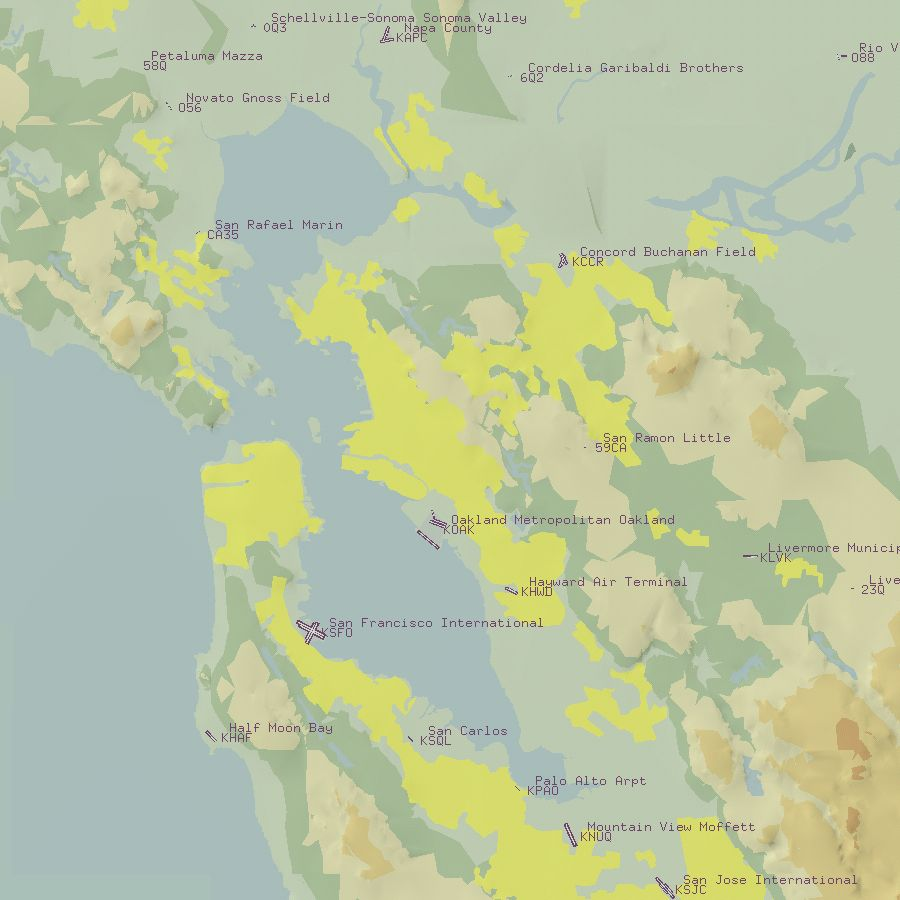
\epsfig{file=atlassan.eps,width=8cm}\end{center}
\caption{Chart of San Diego, California}
\label{fig:atlassan}
\end{figure}
%
%%%%%%%%%%%%%%%%%%%%%%%%%%%%%%%%%%%%%%%%%%%%%%%%%%%%%%%%%%%%%%%%%%
%
\section*{Simulator Status}
%
We have a wide range of people interested and participating in this
project.  This is truly a global effort with contributors from just
about every continent.  Interests range from building a realistic home
simulator out old airplane parts, to university research and
instructional use, to simply having a viable alternative to commercial
PC simulators.  Here are some current uses:
%
\begin{enumerate}
%
\item University of Illinois at Urbana Champaign.
FlightGear is providing a platform for icing research for the Smart
Icing Systems Project.
%
\item Simon Fraser University, British Columbia Ca\-nada.
Portions of FlightGear were used in simulation to develop the needed
control algorithms for an autonomous aerial vehicle.
%
\item Iowa State University.
A senior project intended to retrofit some older sim hardware with
FlightGear based software.
%
\item University of Minnesota - Human Factors Research Lab.
FlightGear brings new life to an old Agwagon single seat, single
engine simulator.
%
%\item Ray Woodworth's Flight Simulator Motion Chair.
%FlightGear provides real-time pitch, roll, and yaw data to
%realistically control this motion chair.
%
\item Aeronautical Development Agency, Bangalore India.
FlightGear is used as as the image generator for a flight simulation
facility for piloted evaluation of ski-jump launch and arrested
recovery of a fighter aircraft from an aircraft carrier.
%
\item Veridian Engineering Division, Buffalo, NY.
FlightGear is used for the scenery and out-the-window view for the
Genesis 3000 flight simulator.
%
\end{enumerate}

Reselling open source software has not been a good revenue source
for other companies, partly because of the rapid version changes
and partly because of the low cost of bandwidth for the consumer.
Yet, several organizations are also considering making retail versions.
Can FlightGear be a viable profit center?

Suppose we separate the database of visual scenery from everything else.
That everything else is only few megabytes, which easily fits into a corner
of a CD and will readily be downloaded whenever a new version becomes available.  
As with many other GUI packages, it will probably be repackaged by the
distributions to ensure a painless installation for the community.
There appears to be little benefit in making a product here,
especially since closed source
flight simulator games are available at under $\$20$.

In contrast, the scenery is more than a
gigabyte for each continent, is unlikely to get any smaller,
and represents a significant download.
The scenery is relatively stable over time, old versions are
usually useful with newer releases of the binary software, and
the upgrades only add detail to an existing and viable database.
There is clearly an opportunity to retail a DVD (or a dozen CDs)
that contain the scenery.  The marginal cost of adding a few
dozen binaries, for popular operating system distributions
 and driver combinations, is probably trivial.
Thus, this retail package is likely to be fully functional.

Alternatively, suppose we consider the pilot's viewpoint.  Most general
aviation aircraft cruise at below 200 knots and flight visibility is
(in real life) usually below 20 miles for the lower altitudes that
are accessible with ordinary non-turbocharged piston engines.
Even when flying in a straight line, a maximum of 8000 square miles
of new terrain will come into view during each hour of flight.
Currently, the database uses about one megabyte for 600 square miles,
so a streaming rate of 12 megabytes/hour will be sufficient.
The rate will be lower when previously-downloaded scenery is in view.

This need not impact the core FlightGear source code.  The latitude
and longitude of the aircraft are already exported for use by
independent programs, so the center of interest is trivially available.
Since the scenery is stored in $100\,km^2$ pieces,
an independent program need only generate a
list of the closest elements that have not been fetched yet,
and issue a {\tt wget} to ensure that they will be available
before the aircraft gets close enough for the pilot to see them.

A 56K modem is capable of 12 megabytes per hour before compression.
If streaming scenery can be delivered essentially through any internet
connection, 
it might remove the market need for retail scenery packages.
Multiplying this bandwidth by a worldwide community of users
will result in a sizeable traffic impact on the distributing servers.
Is the total still going to be low enough to be supported
for goodwill, or will free servers gradually transition to 
monthly access fees and maybe even deliver proprietary content?

% * Business cases involving FGFS, such as retail
%
%%%%%%%%%%%%%%%%%%%%%%%%%%%%%%%%%%%%%%%%%%%%%%%%%%%%%%%%%%%%%%%%%%
%
\section*{Simulating Flight Training}
%
FlightGear could also be helpful when learning to fly aircraft.
Flight training is carefully regulated by the government, to
ensure that aircraft generally stay in the sky until their pilot intends
for them to come down safely.  There are thus some real concerns
which need to be addressed before authorities can approve a system.
%
\begin{enumerate}
%
\item Do the controls feel, and operate, sufficiently like the
ones in the aircraft that a pilot can use them without confusion?
Are they easier to use and/or do they obscure dangerous real-life effects?
%
\item Does the software provide a forward view that is representative
for the desired training environment?
%
\item Are the instruments drawn
such that a pilot can easily read and interpret them as usual?
Do they have the systematic errors that often cause accidents?
%
\item Can all needed cockpit switches and knobs be operated intuitively?
%
\item When operated in the limited envelope of flight configurations
that is applied to the training activity, does it match the
manufacturer's data for the aircraft performance?
%
\item Are the weather settings accessible and intuitive to the instructor?
How about causing system failures and broken instrumentation?
%
\item Can the pilot conduct normal interactions with air traffic control?
Can the instructor easily determine whether the pilot is complying
with the control instructions and record errors for subsequent review?
%
\item Is the pilot's manual for the simulator similar and arrangement
to that of an aircraft, such that it can readily be used in flight?
%
\item Can all maneuvers be performed in the same way as in an aircraft?
%
\end{enumerate}
%
In that (partial) list of concerns, the quality of the actual
flight simulation (which is really what FlightGear is offering)
is a minor topic and and acceptable performance is easily achieved.
In contrast, a large package of documentation must be added to the
software to explain and teach people how to use it correctly.
This has led to a separate project {\tt FGATD}\cite{fgatd},
whose goal is to
initially meet the lowest standard created by the United States
Federal Aviation Administration (FAA).  Don't expect it to finish soon.

It is easy to suggest that the FAA is being unrealistic in requiring
this documentation, but they are responding to important traits
in human nature that won't go away just because they're inconvenient.

For example, the things learnt first leave an almost unshakeable
impression and, at times of severe stress, will over-rule later
training.  Thus, any false impressions that are learned by a
beginning student through using a simulator will tend to remain
hidden until a dangerous and potentially lethal situation is
encountered, at which time the pilot may react wrongly and die.
Pilots who use a simulator on an ongoing basis to hone their skills
will get an excessively optimistic opinion of their skills, if the
simulator is too easy to fly or does not exhibit common flaws.
As a result, they will willingly fly into situations that are
in practice beyond their skill proficiency and be at risk.

Clearly, a flight simulator (such as FlightGear) can only safely
be used for training when under the supervision of a qualified
instructor, who can judge whether the learning experience is beneficial.
The documentation materials are essential to supporting that role.
%
%%%%%%%%%%%%%%%%%%%%%%%%%%%%%%%%%%%%%%%%%%%%%%%%%%%%%%%%%%%%%%%%%%
%
\section*{What's in the future?}
%
As with any Open Source project, there are as many possible futures as there
are users and developers of the code.  Some areas to think about are:

The aerodynamic models are not (yet) accurate enough for use in all
flight situations, so they don't reflect the challenges
and excitement of acrobatic maneuvering.  The models also don't react like
a Cessna 172, which is not designed or certified for such maneuvers.

Surround projectors, head mounted displays, directional sound
and cockpit motion are rapidly converging into consumer technologies.
Maybe we can immerse the users so well that they fly conservatively
because they forget that they're not in real danger.

Recent radar and visual satellite surveys of the earth's surface
have enough detail to be directly used as photorealistic scenery.
But not until someone figures out how to manipulate terabytes in real time,
since the data volume is about a million times larger than now.

The aircraft wake is invisible, can last five minutes, descends slowly
or spreads across the ground, is blown around by the wind and is 
extremely dangerous to following aircraft.  A future extension to 
{\tt fgd} could keep track of the hundreds of miles of wake trails
in a given area and notify individual aircraft when they are encountering
invisible severe turbulence.

Replication and scalability is only starting to take hold in the
desktop environment.  A room of several hundred computers acting
as X terminals for word processing can reboot and, 
within a couple of minutes, all be running
FlightGear identically.  They're ready for the next class of student pilots.
%
%%%%%%%%%%%%%%%%%%%%%%%%%%%%%%%%%%%%%%%%%%%%%%%%%%%%%%%%%%%%%%%%%%
%
\section*{Conclusions}
%
On the surface, FlightGear is a simple Open Source project that
builds on many existing projects in the community traditions.
Due to the subject it addresses, many issues and concerns
are raised that rarely inconvenience most other project teams.
These elements are providing the exciting challenges and variety
of associated activities that the developer team is enjoying.

%%%%%%%%%%%%%%%%%%%%%%%%%%%%%%%%%%%%%%%%%%%%%%%%%%%%%%%%%%%%%%%%%%
%
% References and links
\renewcommand{\refname}{\section*{References}}
\begin{footnotesize}
\begin{thebibliography}{99}
\bibitem{fgfs} \texttt{http://www.flightgear.org/}
\bibitem{plib} \texttt{http://plib.sourceforge.net/}
\bibitem{lsb} \texttt{http://www.linuxbase.org/}
\bibitem{abi} \texttt{http://oss.sgi.com/projects/ogl-sample/ABI/}
\bibitem{gltron} \texttt{http://www.gltron.org/}
\bibitem{jsbsim} \texttt{http://jsbsim.sourceforge.net/}
\bibitem{terragear} \texttt{http://www.terragear.org/}
\bibitem{atlas} \texttt{http://atlas.sourceforge.net/}
\bibitem{fgatd} \texttt{http://fgatd.sourceforge.net/}
\end{thebibliography}
\end{footnotesize}
\hrule
%
%%%%%%%%%%%%%%%%%%%%%%%%%%%%%%%%%%%%%%%%%%%%%%%%%%%%%%%%%%%%%%%%%%
%
% Optional: "About the author"
%
{\footnotesize
About the authors:
\\[0.5mm]
\textsl{Alexander Perry} holds M.A. and Ph.D. degrees in engineering from
Cambridge University in England and currently works
as a senior research engineer for \textsl{Quantum Magnetics} in San Diego.
He is one of the \textsl{FlightGear} developers,
a commercial and instrument rated pilot, ground instructor and
an aviation safety counselor in San Diego and Imperial counties of California.
\\[0.5mm]
\textsl{Curtis Olson} holds a M.S. degree in computer science from
the University of Minnesota.  He currently works as a simulation
engineer at the Human Factors Research Lab of the University of
Minnesota developing and support their research driving simulators.
He is the \textsl{FlightGear} project leader and also a major developer.
}
%
%%%%%%%%%%%%%%%%%%%%%%%%%%%%%%%%%%%%%%%%%%%%%%%%%%%%%%%%%%%%%%%%%%
%
\end{document}

